\section{Rotor aerodynamic and structural design} \label{rotor design}
This section deals with the aerodynamic and the inner structural design of the blades for the on-shore wind turbine to be designed at the tip-speed ratio of $7.67$ and for a rotor diameter of $100.0 \m$, as decided in Section \ref{system design}. 
\subsection{Summary of the design}
\begin{table}[H]
\begin{center} 
\caption{Objectives and boundary conditions}\label{tab:rotordesign2}
\begin{tabular}{ |l|c| } 
\hline
\textbf{Parameter} & \textbf{Value/Description}  \\ 
\hline
Number of blades & 3  \\ 
\hline
Rotor diameter & 100.00 m \\ 
\hline
Design tip speed ratio & 7.67 \\
\hline
\end{tabular} \\
\end{center}
\end{table}

\begin{table}[H]
\begin{center} 
\caption{Objectives and boundary conditions}\label{tab:rotordesign2}
\begin{tabular}{ |l|c| } 
\hline
\textbf{Parameter} & \textbf{Value/Description}  \\ 
\hline
Aerofoil 1 & XX  \\ 
\hline
Min. and max. dimensionless radius r/R for aerofoil 1 & XX \\ 
\hline
Aerofoil 2 & XX \\
\hline
Min. and max. dimensionless radius r/R for aerofoil 2 & XX \\
\hline
Aerofoil 3 & XX \\
\hline
Min. and max. dimensionless radius r/R for aerofoil 3 & XX \\
\hline
Twist offset at tip (= blade pitch angle for optimal operation) & XX \\
\hline
‘Thickness factor’ of the blade laminates & XX \\
\hline
\end{tabular} \\
\end{center}
\end{table}

\begin{figure}[H]
\centering
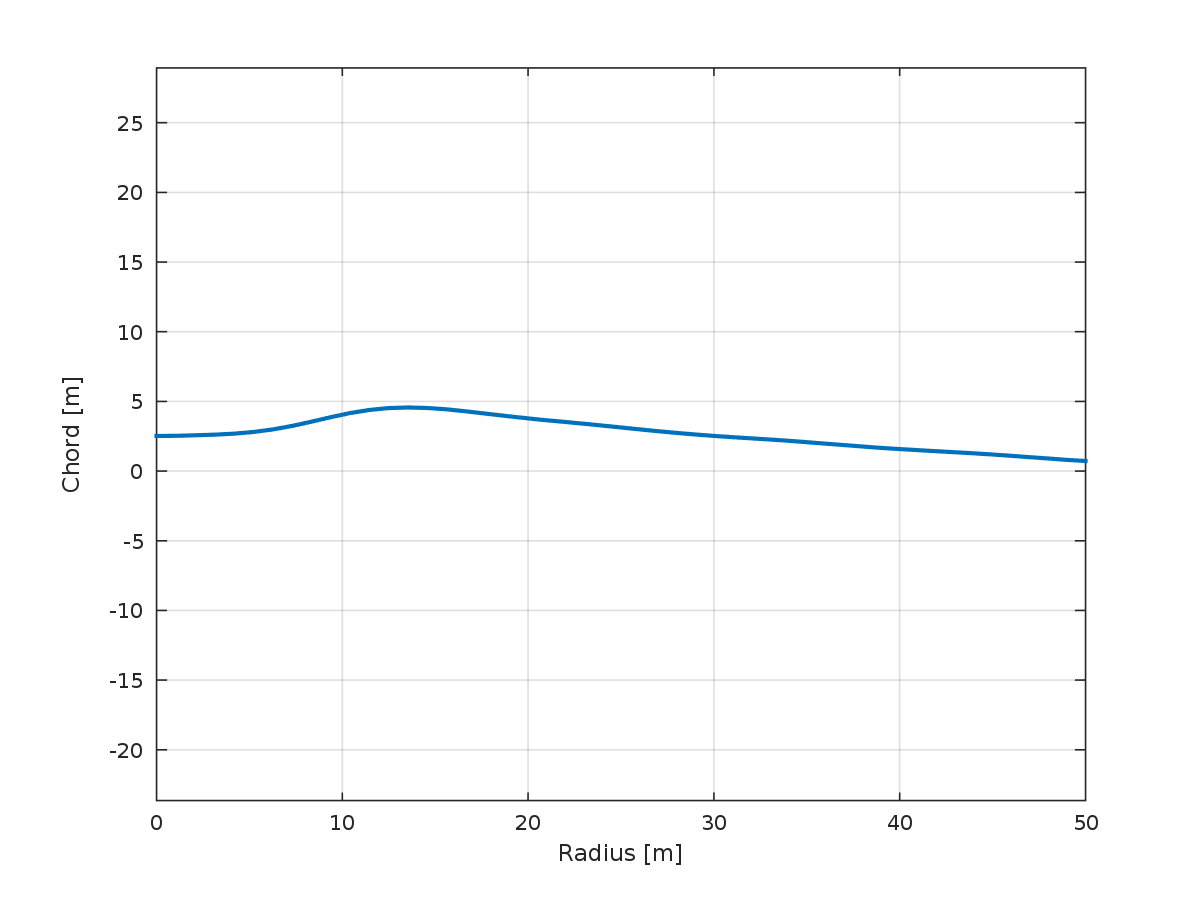
\includegraphics[width=0.7\textwidth]{Images/chord.png} 
\caption{Chord distribution}\label{fig:chord}
\end{figure}

\begin{figure}[H]
\centering
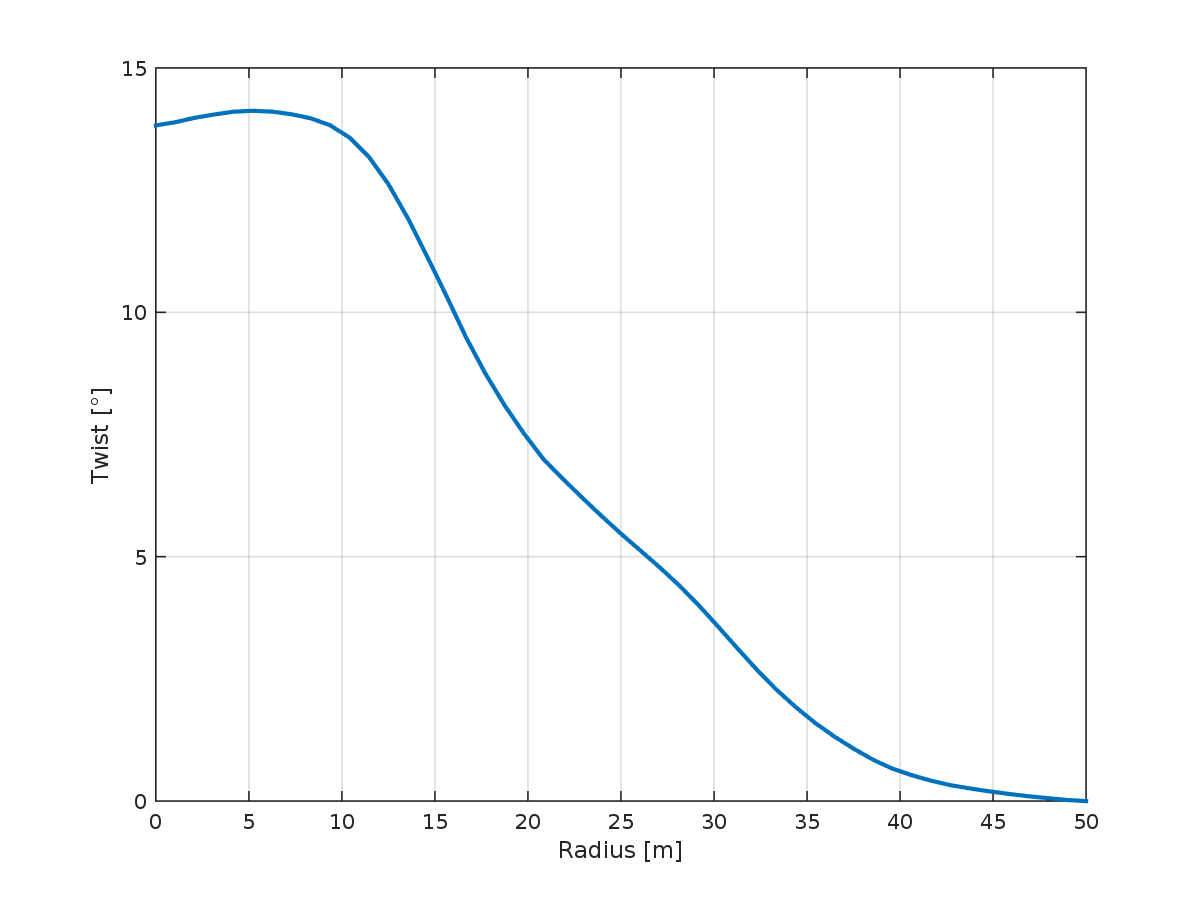
\includegraphics[width=0.7\textwidth]{Images/twist.png} 
\caption{Twist distribution}\label{fig:twist}
\end{figure}


\subsection{Supporting material, analyses and rationale}
The blade from the NREL $5\ MW$ reference turbine \textcolor{red}{(cite this)} is designed using an optimised chord and twist distribution based on its design parameters. The design is then compared with the original reference turbine.

The blade is scaled using the scaling laws from the NREL $5\ MW$ to the desired $2\ MW$ wind turbine. The scaling laws used for each of the parameters have been shown in Table (\textcolor{red}{show table for scaling laws}). These scaling laws are obtained from the square-cube law which states that (\textcolor{red}{state the square-cube law}) and by referring to the scaling laws provided with the course material (\textcolor{red}{cite scaling laws}). The blade's geometry is then optimised to obtain the best desirable performance measured by maximising the power coefficient $C_p$, as can be seen in listing \ref{lst:task3_2} of appendix A.

The optimisation's target is to obtain the twist and chord distribution functions that produce the highest $C_p$ under some constraints. Such functions are expressed by using a set of degrees of freedom, which represent the values of twist and chord at certain uniformly distributed radial locations. The values at all the other locations are obtained by means of cubic spline interpolation. The radial locations used to evaluate the value of $C_p$ are linearly scaled from the reference NREL $5\ MW$ turbine.

The value of $C_p$ is computed by using the BEM code available in the FAST program. Such code has been extracted and isolated as a function that returns the value of $C_p$ given the properties of the wind turbine, as can be seen in listing \ref{lst:Cp}.


\begin{figure}[H]
\centering
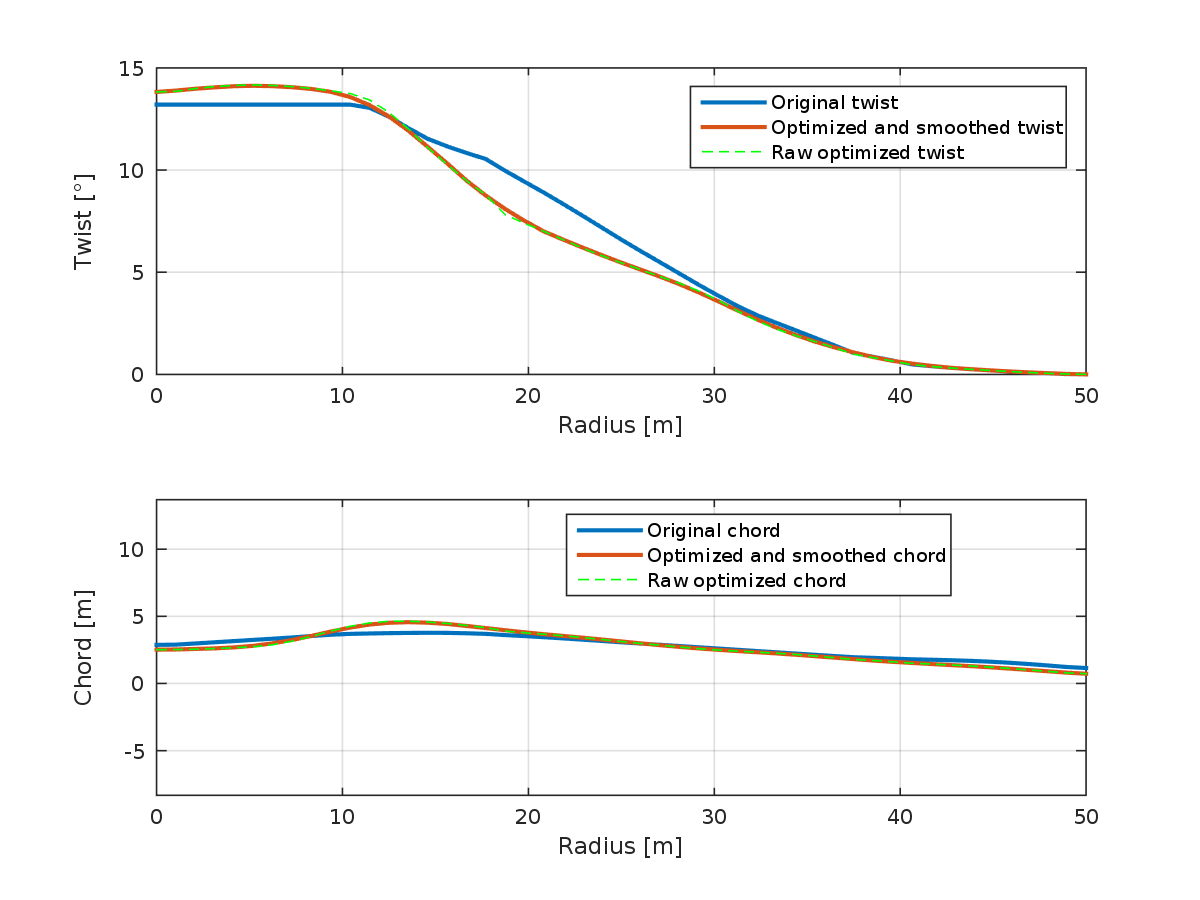
\includegraphics[width=1.0\textwidth]{Images/twist_and_chord.png} 
\caption{Twist distribution}\label{fig:twist_and_chord}
\end{figure}

\textcolor{red}{(TO BE COMPLETED)}


The outer geometry of a rotor blade is thus defined. In order to obtain the interior structure the mass and stiffness of the blades, which make up the structural properties, are scaled from the NREL $5\ MW$ reference turbine using the scaling laws shown in Table (\textcolor{red}{show table for scaling laws}). The scaled blade structural properties are utilised to calculate the tip deflection of the blade designed for the new $2 MW$ wind turbine. In order to calculate the tip deflections both the reference blades and the optimised blades were loaded at a wind speed $v=9.84\ m/s$, which is the rated wind speed for the $2\ MW$ wind turbine.

The tip deflection is calculated using a simple finite element model. The model is based on the Bernoulli beam theory which is applied to the blade modelled as a cantilever beam. The blade discretized using the beam theory is shown in Figure (\textcolor{red}{show beam_theory discretized figure}).The equations for moment and deflection obtained from the Beam theory are applied for each section. Upon using the model the deflections in the flap-wise and the edgewise direction are shown in Figure (\textcolor{red}{show deflection plots}).It can be observed from the plots that, the deflections for the new blade are smaller than that for the reference blade in the flap-wise direction. They are however seen to have increased in the edgewise direction. This is due to the differences in the chord and twist distribution observed between the optimised and the scaled reference blades, as shown in Figure (\textcolor{red}{show deflection comparison plots}). The new chord and twist distributions in the optimised blade cause a redistribution in the inertia in the flap-wise and edgewise directions. Thus, the deflections in the flap-wise and edgewise directions change as a consequence. 

The stresses developed in the flap-wise and edgewise directions in the $5\ MW$ reference and $2\ MW$ optimised turbines are compared relatively by making use of their ratios. The properties that the stresses depend on are namely, the mass $M$ and the stiffness $EI$ along the direction being considered. An additional scaling factor used is the chord $c$ of the respective blades. The chord is utilised to factor in the relative changes in the sizes of the blade cross-sections. The dependence of the stresses for the reference and optimised blades on these factors are expressed as,

\begin{align}
    \sigma_{ref} &\propto \dfrac{M_{ref}}{EI_{ref}}\cdot c_{ref} \label{eq:stress_ref} \\
    \sigma_{opt} &\propto \dfrac{M_{opt}}{EI_{opt}}\cdot c_{opt} \label{eq:stress_opt}
\end{align}

where, $\sigma_{ref},\ M_{ref},\ EI_{ref}$ and $c_{ref}$ represent the stress, mass, stiffness and the chord respectively of the reference blade for the  $5\ MW$ turbine. Similarly, $\sigma_{opt},\ M_{opt},\ EI_{opt}$ and $c_{opt}$ represent the stress, mass, stiffness and the chord respectively of the optimised blade for the  $2\ MW$ turbine being designed. The relationship between the two stresses is established by taking the ratio between Equation \ref{eq:stress_opt} and Equation \ref{eq:stress_ref} and is expressed as,

\begin{equation}
     \zeta = \dfrac{\sigma_{opt}}{\sigma_{ref}} = \dfrac{M_{opt}}{M_{ref}}\cdot\dfrac{EI_{ref}}{EI_{opt}}\cdot \dfrac{c_{opt}}{c_{ref}}
\label{eq:stress_ratio}
\end{equation}

The stress ratio shown in Equation \ref{eq:stress_ratio} is calculated for both the edgewise and the flap-wise directions.